% The contents of this file is 
% Copyright (c)  2010,2011  Charles R. Severance, All Righs Reserved

\chapter{Regular expressions}

So far we have been reading through files, looking for patterns and extracting various bits of lines that we find interesting.  We have been using string methods like {\tt split} and {\tt find} and using lists and string slicing to extract portions of the lines.
\index{regular expressons}
\index{regex}
\index{re module}

This task of searching and extracting is so common that Python has a very powerful library called {\bf regular expressions} that handles many of these tasks quite elegantly.  The reason we have not introduced regular expressions earlier in the book is because while they are very powerful, they are a little complicated and their syntax takes some getting used to. 

Regular expressions are almost their own little programming language for searching and parsing strings.  As a matter of fact, entire books have been written on the topic of regular expressions.  In this chapter, we will only cover the basics of regular expressions.  For more detail on regular expressions, see:

\url{http://en.wikipedia.org/wiki/Regular_expression}

\url{http://docs.python.org/library/re.html}

The regular expression library must be imported into your program before you can use it.  The simplest use of the regular expression library is the {\tt search()} function.  The following program demonstrates a trivial use of the search function.
\index{regex!search}

\beforeverb
\begin{verbatim}
import re
hand = open('mbox-short.txt')
for line in hand:
    line = line.rstrip()
    if re.search('From:', line) :
        print line
\end{verbatim}
\afterverb
%
We open the file, loop through each line and use the regular expression {\tt search()} to only print out lines that contain the string ``From:''.   This program does not use the real power of regular expressions since we could have just as easily used {\tt line.find()} to accomplish the same result.
\index{string!find}

The power of the regular expressions comes when we add to special characters to the search string that allow us to more precisely control which lines match the string.  Adding these special characters to our regular expression allow us to do sophisticated matching and extraction while writing very little code.

For example, the caret character is uses in regular 
expressions to match ``the beginning'' of a line.
We could change our application to only match 
lines where ``From:'' was at the beginning of the line as follows:

\beforeverb
\begin{verbatim}
import re
hand = open('mbox-short.txt')
for line in hand:
    line = line.rstrip()
    if re.search('^From:', line) :
        print line
\end{verbatim}
\afterverb
%
Now we will only match lines that {\em start with} the string ``From:''.  This is still a very simple example that we could have done equivalently with the {\tt startswith()} method from the string library.  But it serves to introduce the notion that regular expressions contain special action characters that give us more control as to what will match the regular expression.
\index{string!startswith}

\section{Character matching in regular expressions}

There are a number of other special characters that let us build even more powerful regular expressions.  The most commonly used special character is the period character which matches any character.
\index{wild card}
\index{regex!wild card}

In the following example, the regular expression ``F..m:'' would match any of the strings ``From:'', ``Fxxm:'', ``F12m:'', or ``F!@m:'' since the period characters in the regular expression match any character.

\beforeverb
\begin{verbatim}
import re
hand = open('mbox-short.txt')
for line in hand:
    line = line.rstrip()
    if re.search('^F..m:', line) :
        print line
\end{verbatim}
\afterverb
%
This is particularly powerful when combined with the ability to indicate that a character can be repeated any number of times using the ``*'' or ``+'' characters in your regular expression.   These special characters mean that instead of matching a single character in the search string they match zero-or-more in the case of the asterisk or one-or-more of the characters in the case of the plus sign.

We can further narrow down the lines that we match using a repeated {\bf wild card} character in the following example:

\beforeverb
\begin{verbatim}
import re
hand = open('mbox-short.txt')
for line in hand:
    line = line.rstrip()
    if re.search('^From:.+@', line) :
        print line
\end{verbatim}
\afterverb
%
The search string ``\verb"^"From:.+@'' will successfully match lines that start with ``From:'' followed by one or more characters ``.+'' followed by an at-sign.  So this will match the following line:

{\tt
{\bf From:}\underline{ stephen.marquard}{\bf @}uct.ac.za
}

You can think of the ``.+'' wildcard as expanding to match all the characters between the 
colon character and the at-sign.  


{\tt
{\bf From:}\underline{.+}{\bf @}
}

It is good to think of the plus and asterisk characters as ``pushy''.  For example the following string would match the last at-sign in the string as the ``.+'' pushes outwards as shown below:

{\tt
{\bf From:}\underline{ stephen.marquard@uct.ac.za, csev@umich.edu, and cwen}{\bf @}iupui.edu
}

It is possible to tell an asterisk or plus-sign not to be so ``greedy'' by adding 
another character.   See the detailed dcumentation for information on turning off the 
greedy behavior.
\index{greedy}

\section{Extracting data using regular expressions}

If we want to extract data from a string in Python we can use the {\tt findall()} method to extract all of the substrings which match a regular expression.  Let's use the example of wanting to extract anything that looks like an e-mail address from any line regardless of format.  For example, we want to pull the e-mail addresses from each of the following lines:

\beforeverb
\begin{verbatim}
From stephen.marquard@uct.ac.za Sat Jan  5 09:14:16 2008
Return-Path: <postmaster@collab.sakaiproject.org>
          for <source@collab.sakaiproject.org>;
Received: (from apache@localhost)
Author: stephen.marquard@uct.ac.za
\end{verbatim}
\afterverb
%
We don't want to write code for each of the types of lines, splitting and slicing differently for each line.  This following program uses {\tt findall()} to find the lines with e-mail addresses in them and extract one or more addresses from each of those lines.
\index{findall}
\index{regex!findall}

\beforeverb
\begin{verbatim}
import re
s = 'Hello from csev@umich.edu to cwen@iupui.edu about the meeting @2PM'
lst = re.findall('\S+@\S+', s)
print lst
\end{verbatim}
\afterverb
%
The {\tt findall()} method searches the string in the second argument and returns a list of all of the strings that look like e-mail addresses.   We are using a special character that indicates a non-whitespace character ({\textbackslash}S). 

The output of the program would be:

\beforeverb
\begin{verbatim}
['csev@umich.edu', 'cwen@iupui.edu']
\end{verbatim}
\afterverb
%
Translating the regular expression, we are looking for substrings that have at least one non-whitespace character, followed by an at-sign, followed by at least one more non-white space characters.  Also, the ``{\textbackslash}S+'' matches as many non-whitespace characters as possible (this is called {\bf ``greedy''} matching in regular expressions).  

The regular expression would match twice (csev@umich.edu and cwen@iupui.edu) but it would not match the string ``@2PM'' because there are no non-blank characters {\em before} the at-sign.  
We can use this regular expression in a program to read all the lines in a file and print out anything that looks like an e-mail address as follows:

\beforeverb
\begin{verbatim}
import re
hand = open('mbox-short.txt')
for line in hand:
    line = line.rstrip()
    x = re.findall('\S+@\S+', line)
    if len(x) > 0 :
        print x
\end{verbatim}
\afterverb
%
We read each line and then extract all the substrings that match our regular expression.  Since {\tt findall()} returns a list, we simple check if the number of elements in our returned list is more than zero to print only lines where we found at least one substring that looks like an e-mail address.

If we run the program on {\tt mbox.txt} we get the following output:

\beforeverb
\begin{verbatim}
['wagnermr@iupui.edu']
['cwen@iupui.edu']
['<postmaster@collab.sakaiproject.org>']
['<200801032122.m03LMFo4005148@nakamura.uits.iupui.edu>']
['<source@collab.sakaiproject.org>;']
['<source@collab.sakaiproject.org>;']
['<source@collab.sakaiproject.org>;']
['apache@localhost)']
['source@collab.sakaiproject.org;']
\end{verbatim}
\afterverb
%
Some of our E-mail addresses have incorrect characters like ``\verb"<"'' or ``;'' at the beginning or end.   Let's declare that we are only interested in the portion of the string that starts and ends with a letter or a number.

To do this, we use another feature of regular expressions.  Square brackets are used to indicate a set of multiple acceptable characters we are willing to consider matching.  In a sense, the ``{\textbackslash}S'' is asking to match the set of ``non-whitespace characters''.  Now we will be a little more explicit in terms of the characters we will match.

Here is our new regular expression:

\beforeverb
\begin{verbatim}
[a-zA-Z0-9]\S*@\S*[a-zA-Z]
\end{verbatim}
\afterverb
%
This is getting a little complicated and you can begin to see why regular expressions are their own little language unto themselves.  Translating this regular expression, we are looking for substrings that start with a {\em single} lowercase letter, upper case letter, or number ``[a-zA-Z0-9]'' followed by zero or more non blank characters ``{\textbackslash}S*'', followed by an at-sign, followed by zero or more non-blank characters ``{\textbackslash}S*'' followed by an upper or lower case letter.  Note that we switched from ``+'' to ``*'' to indicate zero-or-more non-blank characters since ``[a-zA-Z0-9]'' is already one non-blank character.   Remember that the ``*'' or ``+'' applies to the single character immediately to the left of the plus or asterisk.
\index{regex!character sets(brackets)}

If we use this expression in our program, our data is much cleaner:

\beforeverb
\begin{verbatim}
import re
hand = open('mbox-short.txt')
for line in hand:
    line = line.rstrip()
    x = re.findall('[a-zA-Z0-9]\S+@\S+[a-zA-Z]', line)
    if len(x) > 0 :
        print x
\end{verbatim}
\afterverb
%
\beforeverb
\begin{verbatim}
…
['wagnermr@iupui.edu']
['cwen@iupui.edu']
['postmaster@collab.sakaiproject.org']
['200801032122.m03LMFo4005148@nakamura.uits.iupui.edu']
['source@collab.sakaiproject.org']
['source@collab.sakaiproject.org']
['source@collab.sakaiproject.org']
['apache@localhost']
\end{verbatim}
\afterverb
%
Notice that on the ``source@collab.sakaiproject.org'' lines, our regular expression eliminated two letters at the end of the string (``\verb">";'').  This is because when we append ``[a-zA-Z]'' to the end of our regular expression, we are demanding that whatever string the regular expression parser finds, it must end with a letter.   So when it sees the ``\verb">"'' after ``sakaiproject.org\verb">";'' it simply stops at the last ``matching'' letter it found (i.e. the ``g'' was the last good match).

Also note that the output of the program is a Python list that has a string as the single element in the list.

\section{Combining searching and extracting}

If we want to find numbers on lines that start with the string ``X-'' such as:

\beforeverb
\begin{verbatim}
X-DSPAM-Confidence: 0.8475
X-DSPAM-Probability: 0.0000  
\end{verbatim}
\afterverb
%
We don't just want any floating point numbers from any lines.  We only to extract numbers from lines that have the above syntax.

We can construct the following regular expression to select the lines:

\beforeverb
\begin{verbatim}
^X-.*: [0-9.]+
\end{verbatim}
\afterverb
%
Translating this, we are saying, we want lines that start with ``X-'' followed by zero or more characters ``.*'' followed by a colon (``:'') and then a space.  After the space we are looking for one or more characters that are either a digit (0-9) or a period ``[0-9.]+''.  Note that in between the square braces, the period matches an actual period (i.e. it is not a wildcard between the square brackets).

This is a very tight expression that will pretty much match only the lines we are interested in as follows:

\beforeverb
\begin{verbatim}
import re
hand = open('mbox-short.txt')
for line in hand:
    line = line.rstrip()
    if re.search('^X\S*: [0-9.]+', line) :
        print line
\end{verbatim}
\afterverb
%
When we run the program, we see the data nicely filtered to show 
only the lines we are looking for.

\beforeverb
\begin{verbatim}
X-DSPAM-Confidence: 0.8475
X-DSPAM-Probability: 0.0000
X-DSPAM-Confidence: 0.6178
X-DSPAM-Probability: 0.0000
\end{verbatim}
\afterverb
%
But now we have to solve the problem of extracting the numbers using {\tt split}.  While it would be simple enough to use {\tt split}, we can use another feature of regular expressions to both search and parse the line at the same time.
\index{string!split}

Parentheses are another special character in regular expressions.  When you add parentheses to a regular expression they are ignored when matching the string, but when you are using {\tt findall()}, parentheses indicate that while you want the whole expression to match, you only are interested in extracting a portion of the substring that matches the regular expression.  
\index{regex!parentheses}
\index{parentheses!regular expression}

So we make the following change to our program:

\beforeverb
\begin{verbatim}
import re
hand = open('mbox-short.txt')
for line in hand:
    line = line.rstrip()
    x = re.findall('^X\S*: ([0-9.]+)', line)
    if len(x) > 0 :
        print x
\end{verbatim}
\afterverb
%
Instead of calling {\tt search()}, we add parentheses around the part of the regular expression that represents the floating point number to indicate we only want {\tt findall()} to give us back the floating point number portion of the matching string.

The output from this program is as follows:

\beforeverb
\begin{verbatim}
['0.8475']
['0.0000']
['0.6178']
['0.0000']
['0.6961']
['0.0000']
..
\end{verbatim}
\afterverb
%
The numbers are still in a list and need to be converted from strings to floating point but we have used the power of regular expressions to both search and extract the information we found interesting.

As another example of this technique, if 
you look at the file there are a number of lines of the form:

\beforeverb
\begin{verbatim}
Details: http://source.sakaiproject.org/viewsvn/?view=rev&rev=39772
\end{verbatim}
\afterverb
%
If we wanted to extract all of the revision numbers (the integer number at the end of these lines) using the same technique as above,  we could write the following program:

\beforeverb
\begin{verbatim}
import re
hand = open('mbox-short.txt')
for line in hand:
    line = line.rstrip()
    x = re.findall('^Details:.*rev=([0-9.]+)', line)
    if len(x) > 0:
        print x
\end{verbatim}
\afterverb
%
Translating our regular expression, we are looking for lines that start with ``Details:', followed by any any number of characters ``.*'' followed by ``rev='' and then by one or more digits.   We want lines that match the entire expression but we only want to extract the integer number at the end of the line so we surround ``[0-9]+'' with parentheses.  

When we run the program, we get the following output:

\beforeverb
\begin{verbatim}
['39772']
['39771']
['39770']
['39769']
...
\end{verbatim}
\afterverb
%
Remember that the ``[0-9]+'' is ``greedy'' and it tries to make as large a string of digits as possible before extracting those digits.  This ``greedy'' behavior is why we get all five digits for each number.  The regular expression library expands in both directions until it counters a non-digit, the beginning, or the end of a line.

Now we can use regular expressions to re-do an exercise from earlier in the book where we were interested in the time of day of each mail message.   We looked for lines of the form:

\beforeverb
\begin{verbatim}
From stephen.marquard@uct.ac.za Sat Jan  5 09:14:16 2008
\end{verbatim}
\afterverb
%
And wanted to extract the hour of the day for each line.  Previously we did this with two calls to {\tt split}.  First the line was split into words and then we pulled out the fifth word and split it again on the colon character to pull out the two characters we were interested in.

% Add a section on the notion of brittle code
While this worked, it actually results in pretty brittle code that is assuming the lines are nicely formatted.  If you were to add enough error checking (or a big try/except block) to insure that your program never failed when presented with incorrectly formatted lines, the code would balloon to 10-15 lines of code that was pretty hard to read.

We can do this far simpler with the following regular expression:

\beforeverb
\begin{verbatim}
^From .* [0-9][0-9]:
\end{verbatim}
\afterverb
%
The translation of this regular expression is that we are looking for lines that start with ``From '' (note the space) followed by any number of characters ``.*'' followed by a space followed by two digits ``[0-9][0-9]'' followed by a colon character.  This is the definition of the kinds of lines we are looking for.  

In order to pull out only the hour using {\tt findall()}, we add parentheses around the two digits as follows:

\beforeverb
\begin{verbatim}
^From .* ([0-9][0-9]):
\end{verbatim}
\afterverb
%
This results in the following program:

\beforeverb
\begin{verbatim}
import re
hand = open('mbox-short.txt')
for line in hand:
    line = line.rstrip()
    x = re.findall('^From .* ([0-9][0-9]):', line)
    if len(x) > 0 : print x
\end{verbatim}
\afterverb
%
When the program runs, it produces the following output:

\beforeverb
\begin{verbatim}
['09']
['18']
['16']
['15']
…
\end{verbatim}
\afterverb
%
\section{Escape character}

Since we use special characters in regular expressions to match the beginning or end of 
a line or specify wild cards, we need a way to indicate that these characters are ``normal'' 
and we want to match the actual character such as a dollar-sign or caret.

We can indicate that we want to simply match a character by prefixing that character 
with a backslash.  For example, we can find money amounts with the following regular
expression.

\beforeverb
\begin{verbatim}
import re
x = 'We just received $10.00 for cookies.'
y = re.findall('\$[0-9.]+',x)
\end{verbatim}
\afterverb
%
Since we prefix the dollar-sign with a backslash, it actually matches the dollar-sign
in the input string instead of matching the ``end of line'' and the rest of the regular
expression matches one or more digits or the period character.  {\em Note:} In between 
square brackets, characters are not ``special''.   So when we say ``[0-9.]'', it really 
means digits or a period.    Outside of square brackets, a period is the ``wild-card'' 
character and matches any character.  In between square brackets, the period is a period.

\section{Summary}

While this only scratched the surface of regular expressions, we have learned a bit about the language of regular expressions.  They are search strings that have special characters in them that communicate your wishes to the regular expression system as to what defines ``matching'' and what is extracted from the matched strings.  Here are some of those special characters and character sequences:

\verb"^" \newline
Matches the beginning of the line.

\$ \newline
Matches the end of the line.

. \newline
Matches any character (a wildcard).

{\textbackslash}s \newline
Matches a whitespace character.

{\textbackslash}S \newline
Matches a non-whitespace character (opposite of {\textbackslash}s).

* \newline
Applies to the immediately preceding character and indicates to match zero or more of the preceding character.

*? \newline
Applies to the immediately preceding character and indicates to match zero or more of the preceding character in ``non-greedy mode''.

+ \newline
Applies to the immediately preceding character and indicates to match zero or more of the preceding character.

+? \newline
Applies to the immediately preceding character and indicates to match zero or more of the preceding character in ``non-greedy mode''.

[aeiou] \newline
Matches a single character as long as that character is in the specified set.  In this example, it would match ``a'', ``e'', ``i'', ``o'' or ``u'' but no other characters.

[a-z0-9] \newline
You can specify ranges of characters using the minus sign.  This example is a single character that must be a lower case letter or a digit.

[\verb"^"A-Za-z] \newline
When the first character in the set notation is a caret, it inverts the logic.  This example matches a single character that is anything {\em other than} an upper or lower case character.

( ) \newline
When parentheses are added to a regular expression, they are ignored for the purpose of matching, but allow you to extract a particular subset of the matched string rather than the whole string when using {\tt findall()}.

{\textbackslash}b \newline
Matches the empty string, but only at the start or end of a word.

{\textbackslash}B \newline
Matches the empty string, but not at the start or end of a word.

{\textbackslash}d \newline
Matches any decimal digit; equivalent to the set [0-9].

{\textbackslash}D \newline
Matches any non-digit character; equivalent to the set [\verb"^"0-9].

\section{Bonus section for UNIX users}

Support for searching files using regular expressions was built into the UNIX operating system 
since the 1960's and it is available in nearly all programming languages in one form or another.

As a matter of fact, there is a command-line program built into UNIX 
called {\bf grep} (Generalized Regular Expression Parser) that does pretty much 
the same as the {\tt search()} examples in this chapter.  So if you have a 
Macintosh or Linux system, you can try the following commands in your command line window.

\beforeverb
\begin{verbatim}
$ grep '^From:' mbox-short.txt
From: stephen.marquard@uct.ac.za
From: louis@media.berkeley.edu
From: zqian@umich.edu
From: rjlowe@iupui.edu
\end{verbatim}
\afterverb
%
This tells {\tt grep} to show you lines that start with the string ``From:'' in the file {\tt mbox-short.txt}.   If you experiment with the {\tt grep} command a bit and read the documentation for {\tt grep}, you will find some subtle differences between the regular expression support in Python and the regular expression support in {\tt grep}.  As an example, {\tt grep} does not support the non-blank character ``{\textbackslash}S'' so you will need to use the slightly more complex set notation ``[\verb"^" ]''- which simply means - match a character that is anything other than a space.

\section{Debugging}

Python has some simple and rudimentary built-in documentation that can be quite helpful if you need a quick refresher to trigger your memory about the exact name of a particular method.   This documentation can be viewed in the Python interpreter in interactive mode.

You can bring up an interactive help system using {\tt help()}.

\beforeverb
\begin{verbatim}
>>> help()

Welcome to Python 2.6!  This is the online help utility.

If this is your first time using Python, you should definitely check out
the tutorial on the Internet at http://docs.python.org/tutorial/.

Enter the name of any module, keyword, or topic to get help on writing
Python programs and using Python modules.  To quit this help utility and
return to the interpreter, just type "quit".

To get a list of available modules, keywords, or topics, type "modules",
"keywords", or "topics".  Each module also comes with a one-line summary
of what it does; to list the modules whose summaries contain a given word
such as "spam", type "modules spam".

help> modules
\end{verbatim}
\afterverb
%
If you know what module you want to use, you can use the {\tt dir()} command to find the methods in the module as follows:

\beforeverb
\begin{verbatim}
>>> import re
>>> dir(re)
[.. 'compile', 'copy_reg', 'error', 'escape', 'findall', 
'finditer', 'match', 'purge', 'search', 'split', 'sre_compile', 
'sre_parse', 'sub', 'subn', 'sys', 'template']
\end{verbatim}
\afterverb
%
You can also get a small amount of documentation on a particular method using the dir command.

\beforeverb
\begin{verbatim}
>>> help (re.search)
Help on function search in module re:

search(pattern, string, flags=0)
    Scan through string looking for a match to the pattern, returning
    a match object, or None if no match was found.
>>> 
\end{verbatim}
\afterverb
%
The built in documentation is not very extensive, but it can be helpful when you are in a hurry
or don't have access to a web browser or search engine.

\section{Glossary}

\begin{description}

\item[brittle code:]
Code that works when the input data is in a particular format but prone to breakage
if there is some deviation from the correct format.  We call this ``brittle code'' 
because it is easily broken.

\item[greedy matching:]
The notion that the ``+'' and ``*'' characters in a regular expression expand outward to match the largest possible string.
\index{greedy}
\index{greedy matching}

\item[grep:]
A command available in most UNIX systems that searches through text files looking for lines that match regular expressions.  The command name stands for "Generalized Regular Expression Parser".
\index{grep}

\item[regular expression:]
A language for expressing more complex search strings.  A regular expression may contain special characters that indicate that a search only matches at the beginning or end of a line or many other similar capabilities.

\item[wild card:]
A special character that matches any character.   In regular expressions the wild card character is the period character.
\index{wild card}

\end{description}

\section{Exercises}

\begin{ex}
Write a simple program to simulate the operation of the the {\tt grep} command 
on UNIX.  Ask the user to enter a regular expression and count the number
of lines that matched the regular expression:

\beforeverb
\begin{verbatim}
$ python grep.py
Enter a regular expression: ^Author
mbox.txt had 1798 lines that matched ^Author

$ python grep.py
Enter a regular expression: ^X-
mbox.txt had 14368 lines that matched ^X-

$ python grep.py
Enter a regular expression: java$
mbox.txt had 4218 lines that matched java$
\end{verbatim}
\afterverb
%
\end{ex}

\begin{ex}
Write a program to look for lines of the form

\verb"New Revision: 39772"

And extract the number from each of the lines using a regular expression
and the {\tt findall()} method.  Compute the average of the numbers and 
print out the average.
\end{ex}

\chapter{Networked programs}

While many of the examples in this book have focused on reading
files and looking for data in those files, there are many different
sources of information when one considers the Internet.

In this chapter we will pretend to be a web browser and retrieve web
pages using the HyperText Transport Protocol (HTTP).  Then we will read
through the web page data and parse it.

\section{HyperText Transport Protocol - HTTP}

The network protocol that powers the web is actually quite simple and 
there is built-in support in Python called {\tt sockets} which makes it very 
easy to make network connections and retrieve data over those
sockets in a Python program.

A {\bf socket} is much like a file, except that it 
provides a two-way connection between two 
programs with a single socket.  
You can both read from and write to the same socket.  If you write something to 
a socket it is sent to the application at the other end of the socket.  If you 
read from the socket, you are given the data which the other application has sent.

But if you try to read a socket when the program on the other end of the socket
has not sent any data - you just sit and wait.  If the programs on both ends
of the socket simply wait for some data without sending anything, they will wait for
a very long time.

So an important part of programs that communicate over the Internet is to have some
sort of protocol.   A protocol is a set of precise rules that determine who
is to go first, what they are to do, and then what are the responses to that message,
and who sends next and so on.  In a sense the two applications at either end 
of the socket are doing a dance and making sure not to step on each other's toes.

There are many documents which describe these network protocols.  The HyperText Transport 
Protocol is described in the following document:

\url{http://www.w3.org/Protocols/rfc2616/rfc2616.txt}

This is a long and complex 176 page document with a lot of detail.  If you 
find it interesting feel free to read it all.  But if you take a look around page 36 of
RFC2616 you will find the syntax for the GET request.  If you read in detail, you will
find that to request a document from a web server, we make a connection to 
the {\tt www.py4inf.com} server on port 80, and then send a line of the form:

{\tt GET http://www.py4inf.com/code/romeo.txt HTTP/1.0 }

Where the second parameter is the web page we are requesting and then 
we also send a blank line.  The web server will respond with some 
header information about the document and a blank line
followed by the document content.

\section{The World's Simplest Web Browser}

Perhaps the easiest way to show how the HTTP protocol works is to write a very 
simple Python program that makes a connection to a web server and following
the rules of the HTTP protocol, requests a document 
and displays what the server sends back.

\beforeverb
\begin{verbatim}
import socket

mysock = socket.socket(socket.AF_INET, socket.SOCK_STREAM)
mysock.connect(('www.py4inf.com', 80))
mysock.send('GET http://www.py4inf.com/code/romeo.txt HTTP/1.0\n\n')

while True:
    data = mysock.recv(512)
    if ( len(data) < 1 ) :
        break
    print data

mysock.close()
\end{verbatim}
\afterverb
%
First the program makes a connection to port 80 on 
the server \url{www.py4inf.com}.
Since our program is playing the role of the ``web browser'' the HTTP
protocol says we must send the GET command followed by a blank line.

\beforefig
\centerline{\includegraphics[height=1.50in]{figs2/socket.eps}}
\afterfig

Once we send that blank line, we write a loop that receives data 
in 512 character chunks from the socket and prints the data out 
until there is no more data to read (i.e. the recv() returns 
an empty string).

The program produces the following output:

\beforeverb
\begin{verbatim}
HTTP/1.1 200 OK
Date: Sun, 14 Mar 2010 23:52:41 GMT
Server: Apache
Last-Modified: Tue, 29 Dec 2009 01:31:22 GMT
ETag: "143c1b33-a7-4b395bea"
Accept-Ranges: bytes
Content-Length: 167
Connection: close
Content-Type: text/plain

But soft what light through yonder window breaks
It is the east and Juliet is the sun
Arise fair sun and kill the envious moon
Who is already sick and pale with grief
\end{verbatim}
\afterverb
%
The output starts with headers which the web server sends
to describe the document.
For example, the {\tt Content-Type } header indicated that
the document is a plain text document ({\tt text/plain}).

After the server sends us the headers, it adds a blank line
to indicate the end of the headers and then sends the actual
data of the file {\tt romeo.txt}.

This example shows how to make a low-level network connection
with sockets.   Sockets can be used to communicate with a web
server or with a mail server or many other kinds of servers.
All that is needed is to find the document which describes
the protocol and write the code to send and receive the data
according to the protocol.

However, since the protocol that we use most commonly is
the HTTP (i.e. the web) protocol, Python has a special 
library specifically designed to support the HTTP protocol 
for the retrieval of
documents and data over the web.

\section{Retrieving web pages with {\tt urllib}}

The {\tt urllib} library makes it very easy to retrieve
web pages and process the data in Python.   Using {\tt urllib}
you can treat a web page much like a file.   You simply
indicate which web page you would like to retrieve and
{\tt urllib} handles all of the HTTP protocol details.

The equivalent code to read the {\tt romeo.txt} file
from the web using {\tt urllib} is as follows:

\beforeverb
\begin{verbatim}
import urllib

fhand = urllib.urlopen('http://www.py4inf.com/code/romeo.txt')
for line in fhand:
   print line.strip()
\end{verbatim}
\afterverb
%
Once the web page has been opened with 
{\tt urllib.urlopen} we can treat it like 
a file and read through it using a 
{\tt for} loop.   

When the program runs, we only see the output
of the contents of the file.   The headers
are still sent, but the {\tt urllib} code
consumes the headers and only returns the 
data to us.

\beforeverb
\begin{verbatim}
But soft what light through yonder window breaks
It is the east and Juliet is the sun
Arise fair sun and kill the envious moon
Who is already sick and pale with grief
\end{verbatim}
\afterverb
%

As an example, we can write 
a program to retrieve the data for
{\tt romeo.txt} and compute the frequency
of each word in the file as follows:

\beforeverb
\begin{verbatim}
import urllib

counts = dict()
fhand = urllib.urlopen('http://www.py4inf.com/code/romeo.txt')
for line in fhand:
    words = line.split()
    for word in words:
        counts[word] = counts.get(word,0) + 1   
print counts
\end{verbatim}
\afterverb
%
Again, once we have opened the web page, 
we can read it like a local file.

\section{Parsing HTML and scraping the web}
\index{web!scraping}
\index{parsing HTML}

One of the common uses of the {\tt urllib} capability in Python is 
to {\bf scrape} the web.   Web scraping is when we write a program
that pretends to be a web browser and retrieves pages and then 
examines the data in those pages looking for patterns.

As an example, a search engine such as Google will look at the source 
of one web page and extract the links to other pages and retrieve
those pages, extracting links, and so on.   Using this technique,
Google {\bf spiders} its way through nearly all of the pages on 
the web.   

Google also uses the frequency of links from pages it finds 
to a particular page as one measure of how ``important'' 
a page is and how highly the page should appear in its search results.

\section{Parsing HTML using Regular Expressions}

One simple way to parse HTML is to use regular expressions to repeatedly
search and extract for substrings that match a particular pattern.

Here is a simple web page:

\beforeverb
\begin{verbatim}
<h1>The First Page</h1>
<p>
If you like, you can switch to the
<a href="http://www.dr-chuck.com/page2.htm">
Second Page</a>.
</p>
\end{verbatim}
\afterverb
%
We can construct a well-formed regular expression to match
and extract the link values from the above text as follows:

\beforeverb
\begin{verbatim}
href="http://.+?"
\end{verbatim}
\afterverb
%
Our regular expression looks for strings that start with
``href="http://'' followed by one or more characters
``.+?'' followed by another double quote.  The question mark 
added to the ``.+?'' indicates that the match is to be done
in a ``non-greedy'' fashion instead of a ``greedy'' fashion.  
A non-greedy match tries to find the {\em smallest} possible matching
string and a greedy match tries to find the {\em largest} possible
matching string.
\index{greedy}
\index{non-greedy}

We need to add parentheses to our regular expression to indicate
which part of our matched string we would like to extract and
produce the following program:
\index{regex!parentheses}
\index{parentheses!regular expression}

\beforeverb
\begin{verbatim}
import urllib
import re

url = raw_input('Enter - ')
html = urllib.urlopen(url).read()
links = re.findall('href="(http://.*?)"', html)
for link in links:
    print link
\end{verbatim}
\afterverb
%
The {\tt findall} regular expression method will give us a list of all
of the strings that match our regular expression, returning only
the link text between the double quotes.

When we run the program, we get the following output:

\beforeverb
\begin{verbatim}
python urlregex.py 
Enter - http://www.dr-chuck.com/page1.htm
http://www.dr-chuck.com/page2.htm

python urlregex.py 
Enter - http://www.py4inf.com/book.htm
http://www.greenteapress.com/thinkpython/thinkpython.html
http://allendowney.com/
http://www.py4inf.com/code
http://www.lib.umich.edu/espresso-book-machine
http://www.py4inf.com/py4inf-slides.zip
\end{verbatim}
\afterverb
%
Regular expressions work very nice when your HTML is well-formatted
and predictable.  But since there is a lot of ``broken'' HTML pages
out there, you might find that a solution only using 
regular expressions might either miss some valid links or end up 
with bad data.

This can be solved by using a robust HTML parsing library.

\section{Parsing HTML using BeautifulSoup}
\index{BeautifulSoup}

There are a number of Python libraries which can help you parse
HTML and extract data from the pages.  Each of the libraries
has its strengths and weaknesses and you can pick one based on 
your needs.

As an example, we will simply parse some HTML input 
and extract links using the {\bf BeautifulSoup} library.   
You can download and install the BeautifulSoup code
from:

\url{www.crummy.com}

You can download and ``install'' BeautifulSoup or you 
can simply place the {\tt BeautifulSoup.py} file in the
same folder as your application.

Even though HTML looks like XML and some pages are carefully 
constructed to be XML, most HTML is generally broken in ways
that cause an XML parser to reject the entire page of HTML as
improperly formed.  BeautifulSoup tolerates highly flawed 
HTML and still lets you easily extract the data you need.

We will use {\tt urllib} to read the page and then use
{\tt BeautifulSoup} to extract the {\tt href} attributes from the
anchor ({\tt a}) tags.
\index{BeautifulSoup}
\index{HTML}
\index{parsing!HTML}

\beforeverb
\begin{verbatim}
import urllib
from BeautifulSoup import *

url = raw_input('Enter - ')
html = urllib.urlopen(url).read()
soup = BeautifulSoup(html)

# Retrieve all of the anchor tags
tags = soup('a')
for tag in tags:
   print tag.get('href', None)
\end{verbatim}
\afterverb
%
The program prompts for a web address, then opens the web
page, reads the data and passes the data to the BeautifulSoup
parser, and then retrieves all of the anchor tags and prints
out the {\tt href} attribute for each tag.

When the program runs it looks as follows:

\beforeverb
\begin{verbatim}
python urllinks.py 
Enter - http://www.dr-chuck.com/page1.htm
http://www.dr-chuck.com/page2.htm

python urllinks.py 
Enter - http://www.py4inf.com/book.htm
http://www.greenteapress.com/thinkpython/thinkpython.html
http://allendowney.com/
http://www.si502.com/
http://www.lib.umich.edu/espresso-book-machine
http://www.py4inf.com/code
http://www.pythonlearn.com/
\end{verbatim}
\afterverb
%
You can use BeautifulSoup to pull out various parts of each 
tag as follows:
\beforeverb
\begin{verbatim}
import urllib
from BeautifulSoup import *

url = raw_input('Enter - ')
html = urllib.urlopen(url).read()
soup = BeautifulSoup(html)

# Retrieve all of the anchor tags
tags = soup('a')
for tag in tags:
   # Look at the parts of a tag
   print 'TAG:',tag
   print 'URL:',tag.get('href', None)
   print 'Content:',tag.contents[0]
   print 'Attrs:',tag.attrs
\end{verbatim}
\afterverb
%
This produces the following output:

\beforeverb
\begin{verbatim}
python urllink2.py 
Enter - http://www.dr-chuck.com/page1.htm
TAG: <a href="http://www.dr-chuck.com/page2.htm">
Second Page</a>
URL: http://www.dr-chuck.com/page2.htm
Content: [u'\nSecond Page']
Attrs: [(u'href', u'http://www.dr-chuck.com/page2.htm')]
\end{verbatim}
\afterverb
%
These examples only begin to show the power of BeautifulSoup
when it comes to parsing HTML.  See the documentation 
and samples at
\url{www.crummy.com}
for more detail.

\section{Reading binary files using urllib}

Sometimes you want to retrieve a non-text (or binary) file such as
an image or video file. The data in these files is generally not 
useful to print out but you can easily make a copy of a URL to a local
file on your hard disk using {\tt urllib}.
\index{binary file}

The pattern is to open the URL and use {\tt read} to download the entire
contents of the document into a string variable ({\tt img}) and then write that
information to a local file as follows:

\beforeverb
\begin{verbatim}
img = urllib.urlopen('http://www.py4inf.com/cover.jpg').read()
fhand = open('cover.jpg', 'w')
fhand.write(img)
fhand.close()
\end{verbatim}
\afterverb
%
This program reads all of the data in at once across the network and 
stores it in the variable {\tt img} in the main memory of your computer
and then opens the file {\tt cover.jpg} and writes the data out to your 
disk.  This will work if the size of the file is less than the size
of the memory of your computer.

However if this is a large audio or video file, this program may crash
or ar least run extremly slowly when your computer runs out of memory.
In order to avoid running out of memory, we retrieve the data in blocks
(or buffers) and then write each block to your disk before retrieving
the next block.  This way the program can read any sized file without
using up all of the memory you have in your computer.

\beforeverb
\begin{verbatim}
import urllib

img = urllib.urlopen('http://www.py4inf.com/cover.jpg')
fhand = open('cover.jpg', 'w')
size = 0
while True:
    info = img.read(100000)
    if len(info) < 1 : break
    size = size + len(info)
    fhand.write(info)

print size,'characters copied.'
fhand.close()
\end{verbatim}
\afterverb
%
In this example, we read only 100,000 characters at a time and then 
write those characters to the {\tt cover.jpg} file
before retrieving the next 100,000 characters of data from the
web.

This program runs as follows:

\beforeverb
\begin{verbatim}
python curl2.py 
568248 characters copied.
\end{verbatim}
\afterverb
%

If you have a Unix or Macintosh computer, you probably have a command
built into your operating system that performs this operation
as follows:
\index{curl}

\beforeverb
\begin{verbatim}
curl -O http://www.py4inf.com/cover.jpg
\end{verbatim}
\afterverb
%
The command {\tt curl} is short for ``copy URL'' and so these two 
examples are cleverly named {\tt curl1.py} and {\tt curl2.py} on 
\url{www.py4inf.com/code} as they implement similar functionality
to the {\tt curl} command.  There is also a {\tt curl3.py} sample 
program that does this task a little more effectively in case you
actually want to use this pattern in a program you are writing.

\section{Glossary}

\begin{description}

\item[BeautifulSoup:] A Python library for parsing HTML documents
and extracting data from HTML documents
that compensates for most of the imperfections in the HTML that browsers
generally ignore.
You can download the BeautifulSoup code
from 
\url{www.crummy.com}.
\index{BeautifulSoup}

\item[port:] A number that generally indicates which application 
you are contacting when you make a socket connection to a server.
As an example, web traffic usually uses port 80 while e-mail 
traffic uses port 25.
\index{port}

\item[scrape:] When a program pretends to be a web browser and
retrieves a web page and then looks at the web page content. 
Often programs are following the links in one page to find the next
page so they can traverse a network of pages or a social network.
\index{socket}

\item[socket:] A network connection between two applications
where the applications can send and receive data in either direction.
\index{socket}

\item[spider:] The act of a web search engine retrieving a page and
then all the pages linked from a page and so on until they have 
nearly all of the pages on the Internet which they 
use to build their search index.
\index{spider}

\end{description}

\section{Exercises}

\begin{ex}
Change the socket program {\tt socket1.py} to prompt the user for 
the URL so it can read any web page.  
You can use {\tt split('/')} to break the URL into its component parts
so you can extract the host name for the socket {\tt connect} call.
Add error checking using {\tt try} and {\tt except} to handle the condition where the 
user enters an improperly formatted or non-existant URL.  
\end{ex}

\begin{ex}
Change your socket program so that it counts the number of characters it has received 
and stops displaying any text after it has shown 3000 characters.  The program 
should retrieve the entire document and count the total number of characters 
and display the count of the number of characters at the end of the document.
\end{ex}

\begin{ex}
Use {\tt urllib} to replicate the previous exercise of (1) retrieving the document
from a URL, (2) displaying up to 3000 characters, and (3) counting the overall number
of characters in the document.  Don't worry about the headers for this exercise, simply
show the first 3000 characters of the document contents.
\end{ex}

\begin{ex}
Change the {\tt urllinks.py} program to extract and count 
paragraph (p) tags from the retrieved HTML document and 
display the count of the paragraphs as the 
output of your program.  
Do not display the paragraph text - only count them.
Test your program on several small web pages
as well as some larger web pages.
\end{ex}

\begin{ex}
(Advanced) Change the socket program so that it only shows data after the 
headers and a blank line have been received.  Remember that {\tt recv} is
receiving characters (newlines and all) - not lines.
\end{ex}


\chapter{Using Web Services}

Once it became easy to retrieve documents and parse documents 
over HTTP using programs, it did not take long to develop 
an approach where we started producing documents that were specifically
designed to be consumed by other 
programs (i.e. not HTML to be displayed in a browser).

The most common approach when two programs are exchanging data across 
the web is to exchange the data in a format called the ``eXtensible Markup 
Language'' or XML.  

\section{eXtensible Markup Language - XML}

XML looks very similar to HTML, but XML is more structured 
than HTML.  Here is a sample of an XML document:

\beforeverb
\begin{verbatim}
<person>
  <name>Chuck</name>
  <phone type="intl">
     +1 734 303 4456
   </phone>
   <email hide="yes"/>
</person>
\end{verbatim}
\afterverb
%
Often it is helpful to think of an XML document as a tree structure
where there is a top tag {\tt person} and other tags such as {\tt phone}
are drawn as \emph{children} of their parent nodes.

\beforefig
\centerline{\includegraphics[height=1.50in]{figs2/xml-tree.eps}}
\afterfig

\section{Parsing XML}

Here is a simple application that parses some XML
and extracts some data elements from the XML:

\index{ElementTree}
\index{ElementTree!fromstring}
\index{ElementTree!find}
\beforeverb
\begin{verbatim}
import xml.etree.ElementTree as ET

data = '''
<person>
  <name>Chuck</name>
  <phone type="intl">
     +1 734 303 4456
   </phone>
   <email hide="yes"/>
</person>'''

tree = ET.fromstring(data)
print 'Name:',tree.find('name').text
print 'Attr:',tree.find('email').get('hide')
\end{verbatim}
\afterverb
%
Calling {\tt fromstring} converts the string representation
of the XML into a 'tree' of XML nodes.  When the
XML is in a tree, we have a series of methods which we can call to 
extract portions of data from the XML.  

The {\tt find} function searches through the 
XML tree and retrieves a {\bf node} that matches the specified tag.
Each node can have some text, some attributes (i.e. like hide) and
some ``child'' nodes.   Each node can be the top of a tree of nodes.

\beforeverb
\begin{verbatim}
Name: Chuck
Attr: yes
\end{verbatim}
\afterverb
%
Using an XML parser such as {\tt ElementTree} has the advantage
that while the XML in this example is quite simple, it turns
out that there are many rules regarding valid XML and using 
{\tt ElementTree} allows us to extract data from XML without 
worrying about the rules of XML syntax.

\section{Looping through nodes}

Often the XML has multiple nodes and we need to write a loop
to process all of the nodes.  In the following program, 
we loop through all of the {\tt user} nodes:

\index{ElementTree!findall}
\index{ElementTree!get}
\beforeverb
\begin{verbatim}
import xml.etree.ElementTree as ET

input = '''
<stuff>
    <users>
        <user x="2">
            <id>001</id>
            <name>Chuck</name>
        </user>
        <user x="7">
            <id>009</id>
            <name>Brent</name>
        </user>
    </users>
</stuff>'''

stuff = ET.fromstring(input)
lst = stuff.findall('users/user')
print 'User count:', len(lst)

for item in lst:
    print 'Name', item.find('name').text
    print 'Id', item.find('id').text
    print 'Attribute', item.get('x')
\end{verbatim}
\afterverb
%
The {\tt findall} method retrieves a Python list of sub-trees that
represent the {\tt user} structures in the XML tree.  Then we can 
write a {\tt for} loop that looks at each of the user nodes, and 
prints the {\tt name} and {\tt id} text elements as well as the 
{\tt x} attribute from the {\tt user} node.

\beforeverb
\begin{verbatim}
User count: 2
Name Chuck
Id 001
Attribute 2
Name Brent
Id 009
Attribute 7
\end{verbatim}
\afterverb
%

\section{Application Programming Interfaces (API)}

We now have the ability to exchange data between applications using HyperText
Transport Protocol (HTTP) and a way to represent complex data that we are 
sending back and forth between these applications using eXtensible 
Markup Language (XML).

The next step is to begin to define and document ``contracts'' between 
applications using these techniques. The general name for these 
application-to-application contracts is {\bf Application Program 
Interfaces} or APIs.  When we use an API, generally one program
makes a set of {\bf services} available for use by other applications
and publishes the APIs (i.e. the ``rules'') which must be followed to 
access the services provided by the program.

When we begin to build our programs where the functionality of
our program includes access to services provided by other programs, 
we call the approach a {\bf Service-Oriented Architecture} or SOA.
A SOA approach is one where our overall application makes use of 
the services of other applications.  A non-SOA approach is where the
application is a single stand-alone application which contains all of the
code necessary to implement the application.

We see many examples of SOA when we use the web.  We can go to a single 
web site and book air travel, hotels, and automobiles all from a 
single site.  The data for hotels is not stored on the airline computers. 
Instead, the airline computers contact the services on the hotel computers
and retrieve the hotel data and present it to the user.  When the user
agrees to make a hotel reservation using the airline site, the airline site uses
another web service on the hotel systems to actually make the reservation.
And when it comes to charge your credit card for the whole transaction, 
still other computers become involved in the process.

\beforefig
\centerline{\includegraphics[height=2.50in]{figs2/soa.eps}}
\afterfig

A Service-Oriented Architecture has many advantages including: (1) we 
always maintain only one copy of data - this is particularly important
for things like hotel reservations where we do not want to over-commit
and (2) the owners of the data can set the rules about the use of their 
data.   With these advantages, a SOA system must be carefully designed
to have good performance and meet the user's needs.

When an application makes a set of services in its API available over the web, 
we call these {\bf web services}. 

\section{Twitter web services}

You are probably familiar with the Twitter web site and its
applications \url{http://www.twitter.com}.  Twitter has a very unique
approach to its API/web services in that all of its data is available
to non-Twitter applications using the Twitter API.

Because Twitter has been so liberal in allowing access to its data,
it has enabled thousands of software developers to build their own
customized Twitter-based software.  These additional applications greatly
increase the value of Twitter far beyond simply a web site.  The 
Twitter web services allow the building of whole new applications that
the Twitter team may never have thought of.  It is said that over 90 percent
of the use of Twitter is through the API (i.e. not through the {\tt twitter.com}
web user interface).

You can view the Twitter API documentation at 
\url{http://apiwiki.twitter.com/}.  The Twitter API is an example
of the REST style of web services.
We will focus on the Twitter API
to retrieve a list of a user's friends and their statuses.  As an 
example, you can visit the following URL:

\url{http://api.twitter.com/1/statuses/friends/drchuck.xml}

To see a list of the friends of the twitter account {\tt drchuck}.
It may look like a mess in your browser.   To see the actual XML
returned by Twitter, you can view the source of the returned
``web page''.

We can retrieve this same XML using Python using the {\tt urllib}
utility:

\beforeverb
\begin{verbatim}
import urllib

TWITTER_URL = 'http://api.twitter.com/l/statuses/friends/ACCT.xml'

while True:
    print ''
    acct = raw_input('Enter Twitter Account:')
    if ( len(acct) < 1 ) : break
    url = TWITTER_URL.replace('ACCT', acct)
    print 'Retrieving', url
    document = urllib.urlopen (url).read()
    print document[:250]
\end{verbatim}
\afterverb
%
The program prompts for a Twitter account and opens the URL
for the friends and statuses API and then retrieves the 
text from the URL and shows us the first 250 characters of
the text.

\beforeverb
\begin{verbatim}
python twitter1.py

Enter Twitter Account:drchuck
Retrieving http://api.twitter.com/l/statuses/friends/drchuck.xml
<?xml version="1.0" encoding="UTF-8"?>
<users type="array">
<user>
  <id>115636613</id>
  <name>Steve Coppin</name>
  <screen_name>steve_coppin</screen_name>
  <location>Kent, UK</location>
  <description>Software developing, best practicing, agile e

Enter Twitter Account:
\end{verbatim}
\afterverb
%
In this application, we have retrieved the XML exactly as if it were
an HTML web page.  If we wanted to extract data from the XML, we 
could use Python string functions but this would become pretty complex
as we tried to really start to dig into the XML in detail.

If we were to dump out some of the retrieved XML it would look roughly as follows:

\beforeverb
\begin{verbatim}
<?xml version="1.0" encoding="UTF-8"?>
<users type="array">
  <user>
    <id>115636613</id>
    <name>Steve Coppin</name>
    <screen_name>steve_coppin</screen_name>
    <location>Kent, UK</location>
    <status>
      <id>10174607039</id>
      <source>web</source>
      </status>
  </user>
  <user>
    <id>17428929</id>
    <name>davidkocher</name>
    <screen_name>davidkocher</screen_name>
    <location>Bern</location>
    <status>
      <id>10306231257</id>
      <text>@MikeGrace If possible please post a detailed bug report </text>
    </status>
  </user>
  ...
\end{verbatim}
\afterverb
%
The top level tag is a {\tt users} and there are multiple {\tt user} tags
below within the {\tt users} tag.   There is also a {\tt status} tag below
the {\tt user} tag.  

\section{Handling XML data from an API}

When we receive well-formed XML data from an API, we generally use
an XML parser such as {\tt ElementTree} to extract information from
the XML data.

In the program below, we retrieve the friends and statuses from
the Twitter API and then parse the returned XML to show the first
four friends and their statuses.

\beforeverb
\begin{verbatim}
import urllib
import xml.etree.ElementTree as ET

TWITTER_URL = 'http://api.twitter.com/l/statuses/friends/ACCT.xml'

while True:
    print ''
    acct = raw_input('Enter Twitter Account:')
    if ( len(acct) < 1 ) : break
    url = TWITTER_URL.replace('ACCT', acct)
    print 'Retrieving', url
    document = urllib.urlopen (url).read()
    print 'Retrieved', len(document), 'characters.' 
    tree = ET.fromstring(document)
    count = 0
    for user in tree.findall('user'):
        count = count + 1
        if count > 4 : break
        print user.find('screen_name').text
        status =  user.find('status')
        if status : 
            txt = status.find('text').text
            print '  ',txt[:50]
\end{verbatim}
\afterverb
%
We use the {\tt findall} method to get a list of the {\tt user} 
nodes and loop through the list using a {\tt for } loop.  
For each {\tt user} node, we pull out the text of the \verb"screen_name" node
and then pull out the {\tt status} node.   If there is a {\tt status}
node, we pull out the text of the {\tt text} node and print the first 50 
characters of the status text.

The pattern is pretty straightforward, we use {\tt findall} and {\tt find}
to pull out a list of nodes or a single node and then if a node is a complex
element with more sub-nodes we look deeper into the node until we reach the 
text element that we are interested in.

The program runs as follows:

\beforeverb
\begin{verbatim}
python twitter2.py 

Enter Twitter Account:drchuck
Retrieving http://api.twitter.com/l/statuses/friends/drchuck.xml
Retrieved 193310 characters.
steve_coppin
   Looking forward to some "oh no the markets closed,
davidkocher
   @MikeGrace If possible please post a detailed bug 
hrheingold
   From today's Columbia Journalism Review, on crap d
huge_idea
   @drchuck  #cnx2010 misses you, too.  Thanks for co

Enter Twitter Account:hrheingold
Retrieving http://api.twitter.com/l/statuses/friends/hrheingold.xml
Retrieved 208081 characters.
carr2n
   RT @tysone: Saturday's proclaimation by @carr2n pr
tiffanyshlain
   RT @ScottKirsner: Turning smartphones into a tool 
soniasimone
   @ACCompanyC Funny, smart, cute, and also nice! He 
JenStone7617
   Watching "Changing The Equation: High Tech Answers

Enter Twitter Account:
\end{verbatim}
\afterverb
%
While the code for parsing the XML and extracting the fields
using {\tt ElementTree} takes a few lines to express what 
we are looking for in the XML, it is much simpler than trying 
to use Python string parsing to pull apart the XML and find 
the data elements.

\section{Glossary}

\begin{description}

\item[API:] Application Program Interface - A contract between
applications that defines the patterns of interaction between 
two application components.
\index{API}

\item[ElementTree:] A built-in Python library used to parse XML data.
\index{ElementTree}

\item[XML:] eXtensible Markup Language - A format that allows for 
the markup of structured data.
\index{XML}
\index{eXtensible Markup Language}

\item[REST:] REpresentational State Transfer - A style of Web Services 
that provide access to resources within an application using the HTTP
protocol.
\index{ElementTree}

\item[SOA:] Service Oriented Architecture - when an application is 
made of components connected across a network.
\index{SOA}
\index{Service Oriented Architecture}

\end{description}

\section{Exercises}

\begin{ex}
Change the program that retrieves twitter data 
({\tt twitter2.py}) to also
print out the location for each of the friends
indented under the name by two spaces as follows:

\beforeverb
\begin{verbatim}
Enter Twitter Account:drchuck
Retrieving http://api.twitter.com/l/statuses/friends/drchuck.xml
Retrieved 194533 characters.
steve_coppin
   Kent, UK
   Looking forward to some "oh no the markets closed,
davidkocher
   Bern
   @MikeGrace If possible please post a detailed bug 
hrheingold
   San Francisco Bay Area
   RT @barrywellman: Lovely AmBerhSci Internet & Comm
huge_idea
   Boston, MA
   @drchuck  #cnx2010 misses you, too.  Thanks for co
\end{verbatim}
\afterverb
%
\end{ex}

\chapter{Using databases and Structured Query Language (SQL)}

\section{What is a database?}
\index{database}

A {\bf database} is a file that is organized for storing data.
Most databases are organized like a dictionary in the sense
that they map from keys to values.  The biggest difference
is that the database is on disk (or other permanent storage),
so it persists after the program ends.  Because a database is
stored on permanent storage, it can store far more data than
a dictionary, which is limited to the size of the memory 
in the computer.

\index{database!indexes}
Like a dictionary, database software is designed to keep 
the inserting and accessing of data very fast, even for large
amounts of data.   Database software maintains its performance by 
building {\bf indexes} as data is added to the database
to allow the computer to jump quickly to a particular
entry.

There are many different database systems which are used for a wide
variety of purposes including: Oracle, MySQL, Microsoft SQL Server, 
PostgreSQL, and SQLite.  We focus on SQLite in this book because
it is a very common database and is already built into Python.  
SQLite is designed to be \emph{embedded} into other applications
to provide database support within the application.  For example,
the Firefox browser also uses the SQLite database internally as do 
many other products.

\url{http://sqlite.org/}

SQLite is well suited to some of the data manipulation problems that we 
see in Informatics such as the Twitter spidering application that we 
describe in this chapter.

\section{Database concepts}

When you first look at a database it looks like a 
spreadsheet with multiple sheets.   The primary data structures 
in a database are:
{\bf tables}, {\bf rows}, and {\bf columns}.  

\beforefig
\centerline{\includegraphics[height=1.50in]{figs2/relational.eps}}
\afterfig

In technical descriptions of relational databases the concepts of 
table, row, and column are more formally referred
to as {\bf relation}, {\bf tuple}, and {\bf attribute}, respectively.
We will use the less formal terms in this chapter.

\section{SQLite Database Browser}

While this chapter will focus on using Python to work with data 
in SQLite database files, many operations can be done more
conveniently using a desktop program called the {\bf SQLite
Database Browser} which is freely available from:

\url{http://sourceforge.net/projects/sqlitebrowser/}

Using the browser you can easily create tables, insert data, edit data, 
or run simple SQL queries on the data in the database.

\beforefig
\centerline{\includegraphics[height=3.00in]{figs2/sqlite.eps}}
\afterfig

In a sense, the database browser is similar to a text editor
when working with text files.   When you want to do one or
very few operations on a text file, you can just open it
in a text editor and make the changes you want.   When you have 
many changes that you need to do to a text file, often you 
will write a simple Python program.  You will find the same 
pattern when working with databases.  You will do simple
operations in the database browser and more complex operations
will be most conveniently done in Python.

\section{Creating a database table}

Databases require more defined structure than Python lists 
or dictionaries\footnote{SQLite actually does allow some 
flexibility in the type of data stored in a column,
but we will keep our data types strict in this chapter
so the concepts apply equally to other database systems 
such as MySQL.}.  

When we create a database {\bf table} we
must tell the database in advance the names of each of the
{\bf columns} in the table and the type of data which we are 
planning to store in each {\bf column}.   When the database software
knows the type of data in each column, it can choose the most 
efficient way to store and lookup the data based on the type of
data. 

You can look at the various data types supported by SQLite
at the following url:

\url{http://www.sqlite.org/datatypes.html}

Defining structure for your data up front may seem inconvenient
at the beginning, but the payoff is fast access to your data 
even when the database contains a large amount of data.

The code to create a database file and a table 
named {\tt Tracks} with two columns in the 
database is as follows:

\index{sqlite3 module}
\index{module!sqlite3}
\beforeverb
\begin{verbatim}
import sqlite3

conn = sqlite3.connect('music.db')
cur = conn.cursor()

cur.execute('DROP TABLE IF EXISTS Tracks ')
cur.execute('CREATE TABLE Tracks (title TEXT, plays INTEGER)')

conn.close()
\end{verbatim}
\afterverb
%
\index{connect function}
\index{function!connect}
\index{cursor function}
\index{function!cursor}
The {\tt connect} operation makes a ``connection'' to the database 
stored in the file {\tt music.db} in the current directory.   If
the file does not exist, it will be created.  The reason this
is called a ``connection'' is that sometimes the database is stored
on a separate ``database server'' from the server on which we 
are running our application.  In our simple examples 
the database will just be a local file in the same directory
as the Python code we are running.

A {\bf cursor} is like a file handle that we can use to perform
operations on the data stored in the database.  Calling 
{\tt cursor()} is very similar conceptually to calling
{\tt open()} when dealing with text files.

\beforefig
\centerline{\includegraphics[height=1.50in]{figs2/cursor.eps}}
\afterfig

Once we have the cursor, we can begin to execute 
commands on the contents of the database using the {\tt execute()}
method.

Database commands are expressed in a special language that has 
been standardized across many different database vendors 
to allow us to learn a single database language.   The database
language is called {\bf Structured Query Language} or {\bf SQL}
for short.

\url{http://en.wikipedia.org/wiki/SQL}

In our example, we are executing two SQL commands in our database.
As a convention, we will show the SQL keywords in uppercase 
and the parts of the command that we are adding (such as the
table and column names) will be shown in lowercase.

The first SQL command removes the {\tt Tracks} table from the 
database if it exists.  This pattern is simply to allow us to 
run the same program to create the {\tt Tracks} table over 
and over again without causing an error.  Note that the
{\tt DROP TABLE} command deletes the table and all of its contents
from the database (i.e. there is no ``undo'').

\beforeverb
\begin{verbatim}
cur.execute('DROP TABLE IF EXISTS Tracks ')
\end{verbatim}
\afterverb
%
The second command creates a table named
{\tt Tracks} with a text column named {\tt title}
and an integer column named {\tt plays}.

\beforeverb
\begin{verbatim}
cur.execute('CREATE TABLE Tracks (title TEXT, plays INTEGER)')
\end{verbatim}
\afterverb
%
Now that we have created a table named {\tt Tracks}, we can put some data
into that table using the SQL {\tt INSERT} operation.   Again, we begin
by making a connection to the database and obtaining the {\tt cursor}.
We can then execute SQL commands using the cursor.

The SQL {\tt INSERT} command indicates which table we are using 
and then defines a new row by listing the fields we want to 
include {\tt (title, plays) } followed by the {\tt VALUES} we want
placed in the new row in the table.   We specify the values
as question marks {\tt (?, ?)} to indicate that the actual 
values are passed in as a tuple {\tt ( 'My Way', 15 ) } as the
second parameter to the {\tt execute()} call.

\beforeverb
\begin{verbatim}
import sqlite3

conn = sqlite3.connect('music.db')
cur = conn.cursor()

cur.execute('INSERT INTO Tracks (title, plays) VALUES ( ?, ? )', 
    ( 'Thunderstruck', 20 ) )
cur.execute('INSERT INTO Tracks (title, plays) VALUES ( ?, ? )', 
    ( 'My Way', 15 ) )
conn.commit()

print 'Tracks:'
cur.execute('SELECT title, plays FROM Tracks')
for row in cur :
   print row

cur.execute('DELETE FROM Tracks WHERE plays < 100')
conn.commit()

cur.close()
\end{verbatim}
\afterverb
%
First we {\tt INSERT} two rows into our table and use {\tt commit()} 
to force the data to be written to the database file.

\beforefig
\centerline{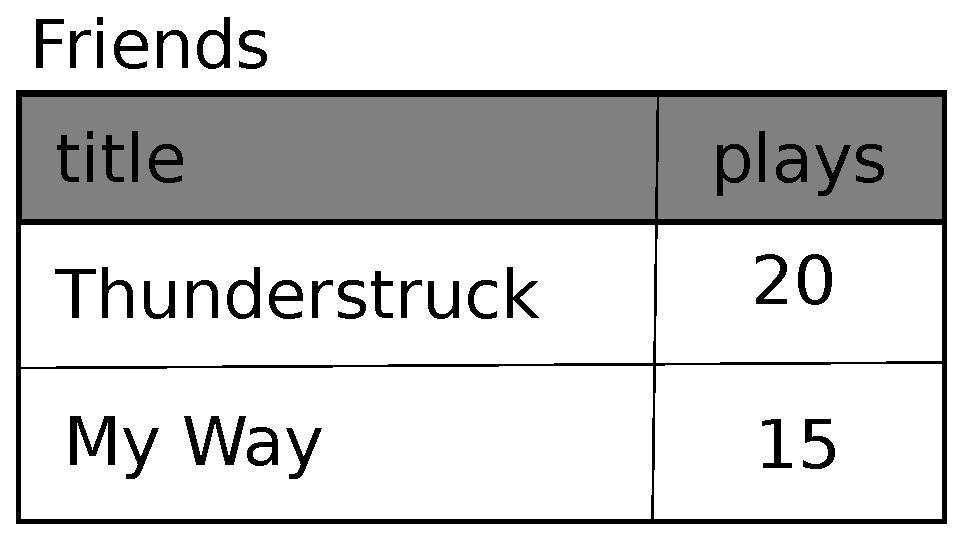
\includegraphics[height=1.00in]{figs2/tracks.eps}}
\afterfig

Then we use the {\tt SELECT} command
to retrieve the rows we just inserted from the table.  
On the 
{\tt SELECT} command, we indicate which columns we would like {\tt (title, plays)}
and indicate which table we want to retrieve the data from.  After we 
execute the {\tt SELECT} statement, the cursor is something we can loop through
in a {\tt for} statement.   For efficiency,
the cursor does not read all of the data from the
database when we execute the {\tt SELECT} statement.  
Instead, the data is read on-demand
as we loop through the rows in the {\tt for} statement.

The output of the program is as follows:

\beforeverb
\begin{verbatim}
Tracks:
(u'Thunderstruck', 20)
(u'My Way', 15)
\end{verbatim}
\afterverb
%
\index{Unicode}
Our {\tt for} loop finds two rows, and each row is a Python tuple with the
first value as the {\tt title} and the second value as the number of {\tt plays}.
Do not be concerned that the title strings are shown starting with 
{\tt u'}.  This is an indication that the strings are {\bf Unicode} strings
that are capable of storing non-Latin character sets.

At the very end of the program, we execute an SQL command to {\tt DELETE} 
the rows we have just created so we can run the program over and over.
The {\tt DELETE} command shows the use of a {\tt WHERE} clause that
allows us to express a selection criterion so that we can ask the database
to apply the command to only the rows that match the criterion.  In this example
the criterion happens to apply to all the rows so we empty the table
out so we can run the program repeatedly.  After the {\tt DELETE} is performed
we also call {\tt commit()} to force the data to be removed from the database.

\section{Structured Query Language (SQL) summary}

So far, we have been using the Structured Query Language in our Python
examples and have covered many of the basics of the SQL commands.
In this section, we look at the SQL language in particular
and give an overview of SQL syntax.

Since there are so many different database vendors, the Structured Query
Language (SQL) was standardized so we could communicate in a portable
manner to database systems from multiple vendors.

A relational database is made up of tables, rows, and columns.  The columns
generally have a type such as text, numeric, or date data.  When we create
a table, we indicate the names and types of the columns:

\beforeverb
\begin{verbatim}
CREATE TABLE Tracks (title TEXT, plays INTEGER)
\end{verbatim}
\afterverb
%
To insert a row into a table, we use the SQL {\tt INSERT} command:

\beforeverb
\begin{verbatim}
INSERT INTO Tracks (title, plays) VALUES ('My Way', 15)
\end{verbatim}
\afterverb
%
The {\tt INSERT} statement specifies the table name, and then a list of
the fields/columns that you would like to set in the new row, and then 
the keyword {\tt VALUES} and then a list of corresponding values 
for each of the fields.

The SQL {\tt SELECT} command is used to retrieve rows and columns from a database.
The {\tt SELECT} statement lets you specify which columns you would
like to retrieve as well as a {\tt WHERE} clause to select which 
rows you would like to see.  It also allows an optional 
{\tt ORDER BY} clause to control the sorting of the returned rows.

\beforeverb
\begin{verbatim}
SELECT * FROM Tracks WHERE title = 'My Way'
\end{verbatim}
\afterverb
%
Using \verb"*" indicates that you want the database to return all of 
the columns for each row that matches the {\tt WHERE} clause.  

Note, unlike in Python, in a SQL {\tt WHERE} clause 
we use a single equal sign 
to indicate a test for equality rather than a double equal sign.
Other logical operations allowed in a {\tt WHERE} clause include 
\verb"<",
\verb">",
\verb"<=",
\verb">=",
\verb"!=",
as well as {\tt AND} and {\tt OR} and parentheses
to build your logical expressions.

You can request that the returned rows be sorted by one of 
the fields as follows:

\beforeverb
\begin{verbatim}
SELECT title,plays FROM Tracks ORDER BY title
\end{verbatim}
\afterverb
%
To remove a row, you need a {\tt WHERE} clause on an SQL {\tt DELETE}
statement.  The {\tt WHERE} clause determines which rows are to be deleted:

\beforeverb
\begin{verbatim}
DELETE FROM Tracks WHERE title = 'My Way'
\end{verbatim}
\afterverb
%
It is possible to {\tt UPDATE} a column or columns within one or more rows
in a table using the SQL {\tt UPDATE} statement as follows:

\beforeverb
\begin{verbatim}
UPDATE Tracks SET plays = 16 WHERE title = 'My Way'
\end{verbatim}
\afterverb
%
The {\tt UPDATE} statement specifies a table and 
then a list of fields and values to change after the {\tt SET} 
keyword and then an optional {\tt WHERE} clause to select
the rows that are to be updated.  A single {\tt UPDATE} statement
will change all of the rows that match the {\tt WHERE} clause, or if 
a {\tt WHERE} clause is not specified, it performs the {\tt UPDATE}
on all of the rows in the table.

These four basic SQL commands (INSERT, SELECT, UPDATE, and DELETE) allow 
the four basic operations needed to create and maintain data.


\section{Spidering Twitter using a database}

In this section, we will create a simple spidering program that will 
go through Twitter accounts and build a database of them.
\emph{Note: Be very careful when running this program.  You do not
want to pull too much data or run the program for too long and
end up having your Twitter access shut off.}

One of the problems of any kind of spidering program is that it 
needs to be able to be stopped and restarted many times and 
you do not want to lose the data that you have retrieved so far.
You don't want to always restart your data retrieval at the
very beginning so we want to store data as we retrieve it so our
program can start back up and pick up where it left off.

We will start by retrieving one person's Twitter friends and their
statuses, looping through the list of friends, and adding each 
of the friends to a database to be retrieved in the future.  After
we process one person's Twitter friends, we check in our database
and retrieve one of the friends of the friend.  We do this over and
over, picking an ``unvisited'' person, retrieving their friend list
and adding friends we have not seen to our list for a future visit.

We also track how many times we have seen a particular friend in the
database to get some sense of ``popularity''.

By storing our list of known accounts and whether 
we have retrieved the account or not, 
and how popular the account is in a database on the disk
of the computer, we can stop and
restart our program as many times as we like.

% TODO: Add a reference to the right spot
This program is a bit complex. It is based on the code 
from the exercise earlier in the book that uses
the Twitter API.

Here is the source code for our Twitter spidering application:

\beforeverb
\begin{verbatim}
import sqlite3
import urllib
import xml.etree.ElementTree as ET

TWITTER_URL = 'http://api.twitter.com/l/statuses/friends/ACCT.xml'

conn = sqlite3.connect('twdata.db')
cur = conn.cursor()

cur.execute('''
CREATE TABLE IF NOT EXISTS 
Twitter (name TEXT, retrieved INTEGER, friends INTEGER)''')

while True:
    acct = raw_input('Enter a Twitter account, or quit: ')
    if ( acct == 'quit' ) : break
    if ( len(acct) < 1 ) :
        cur.execute('SELECT name FROM Twitter WHERE retrieved = 0 LIMIT 1')
        try:
            acct = cur.fetchone()[0]
        except:
            print 'No unretrieved Twitter accounts found'
            continue

    url = TWITTER_URL.replace('ACCT', acct)
    print 'Retrieving', url
    document = urllib.urlopen (url).read()
    tree = ET.fromstring(document)

    cur.execute('UPDATE Twitter SET retrieved=1 WHERE name = ?', (acct, ) )

    countnew = 0
    countold = 0
    for user in tree.findall('user'):
        friend = user.find('screen_name').text
        cur.execute('SELECT friends FROM Twitter WHERE name = ? LIMIT 1', 
            (friend, ) )
        try:
            count = cur.fetchone()[0]
            cur.execute('UPDATE Twitter SET friends = ? WHERE name = ?', 
                (count+1, friend) )
            countold = countold + 1
        except:
            cur.execute('''INSERT INTO Twitter (name, retrieved, friends) 
                VALUES ( ?, 0, 1 )''', ( friend, ) )
            countnew = countnew + 1
    print 'New accounts=',countnew,' revisited=',countold
    conn.commit()

cur.close()
\end{verbatim}
\afterverb
%
Our database is stored in the file {\tt twdata.db} and it has one 
table named {\tt Twitter} and each row in the {\tt Twitter} table
has a column for the account name, whether we have retrieved the friends
of this account, and how many times this account has been ``friended''.

In the main loop of the program, we prompt the user for a Twitter
account name or ``quit'' to exit the program.  
If the user enters a Twitter account, we retrieve the 
list of friends and statuses
for that user and add each friend to the database if 
not already in the database.  If the friend is already in the list, 
we add one to the {\tt friends} field in the row in the database.

If the user presses enter, we look in the database for the next 
Twitter account that we have not yet retrieved and retrieve the
friends and statuses for that account, add them to the database 
or update them and increase their {\tt friends count}.

Once we retrieve the list of friends and statuses, we loop 
through all of the {\tt user} items in the returned XML
and retrieve the \verb"screen_name" for each user.  Then we use
the {\tt SELECT } statement to see if we already have stored this
particular \verb"screen_name" in the database and retrieve the
friend count ({\tt friends}) if the record exists.

\beforeverb
\begin{verbatim}
    countnew = 0
    countold = 0
    for user in tree.findall('user'):
        friend = user.find('screen_name').text
        cur.execute('SELECT friends FROM Twitter WHERE name = ? LIMIT 1', 
            (friend, ) )
        try:
            count = cur.fetchone()[0]
            cur.execute('UPDATE Twitter SET friends = ? WHERE name = ?', 
                (count+1, friend) )
            countold = countold + 1
        except:
            cur.execute('''INSERT INTO Twitter (name, retrieved, friends) 
                VALUES ( ?, 0, 1 )''', ( friend, ) )
            countnew = countnew + 1
    print 'New accounts=',countnew,' revisited=',countold
    conn.commit()
\end{verbatim}
\afterverb
%
Once the cursor executes the {\tt SELECT} statement, 
we must retrieve the rows.  We could do this with a {\tt for} 
statement, but since we are only retrieving
one row ({\tt LIMIT 1}), we can use the {\tt fetchone()} method to fetch the
first (and only) row that is the result of the {\tt SELECT} operation.  
Since {\tt fetchone()} returns the row as a {\bf tuple} (even though there is only
one field), we take the first value from the tuple using {\tt [0]} to get the 
current friend count into the variable {\tt count}.  

If this retrieval is successful, we use the SQL {\tt UPDATE} statement with a 
{\tt WHERE} clause to add one to the {\tt friends} column for the row that 
matches the friend's account.  Notice that there are two placeholders (i.e.
question marks) in the SQL, and the second parameter to the {\tt execute()} is
a two-element tuple which holds the values to be substituted into the SQL
in place of the question marks.

If the code in the {\tt try} block fails it is probably because no record
matched the {\tt WHERE name = ?} clause on the SELECT statement.  So in the
{\tt except} block, we use the SQL {\tt INSERT} statement to add the friend's
\verb"screen_name" to the table with an indication that we have not yet 
retrieved the \verb"screen_name" and setting the friend count to zero.

So the first time the program runs and we enter a Twitter account, the program
runs as follows:
\beforeverb
\begin{verbatim}
Enter a Twitter account, or quit: drchuck
Retrieving http://api.twitter.com/l/statuses/friends/drchuck.xml
New accounts= 100  revisited= 0
Enter a Twitter account, or quit: quit
\end{verbatim}
\afterverb
%
Since this is the first time we have run the program, the database
is empty and we create the database in the file {\tt twdata.db} and
add a table named {\tt Twitter} to the database.  Then we retrieve
some friends and add them all to the database since the database is
empty.

At this point, we might want to write a simple database dumper
to take a look at what is in our {\tt twdata.db} file:
\beforeverb
\begin{verbatim}
import sqlite3

conn = sqlite3.connect('twdata.db')
cur = conn.cursor()
cur.execute('SELECT * FROM Twitter')
count = 0
for row in cur :
   print row
   count = count + 1
print count, 'rows.'
cur.close()
\end{verbatim}
\afterverb
%
This program simply opens the database and selects all of the 
columns of all of the rows in the table {\tt Twitter}, then 
loops through the rows and prints out each row.

If we run this program after the first execution of our Twitter
spider above, its output will be as follows:
\beforeverb
\begin{verbatim}
(u'opencontent', 0, 1)
(u'lhawthorn', 0, 1)
(u'steve_coppin', 0, 1)
(u'davidkocher', 0, 1)
(u'hrheingold', 0, 1)
...
100 rows.
\end{verbatim}
\afterverb
%
We see one row for each \verb"screen_name", that we 
have not retrieved the data for that \verb"screen_name" and 
everyone in the database has one friend.

Now our database reflects the retrieval of the friends of 
our first Twitter account ({\bf drchuck}).  We can run the program
again and tell it to retrieve the friends of the next 
``unprocessed'' account by simply pressing enter instead of
a Twitter account as follows:
\beforeverb
\begin{verbatim}
Enter a Twitter account, or quit: 
Retrieving http://api.twitter.com/l/statuses/friends/opencontent.xml
New accounts= 98  revisited= 2
Enter a Twitter account, or quit: 
Retrieving http://api.twitter.com/l/statuses/friends/lhawthorn.xml
New accounts= 97  revisited= 3
Enter a Twitter account, or quit: quit
\end{verbatim}
\afterverb
%
Since we pressed enter (i.e. we did not specify a Twitter account),
the following code is executed:
\beforeverb
\begin{verbatim}
    if ( len(acct) < 1 ) :
        cur.execute('SELECT name FROM Twitter WHERE retrieved = 0 LIMIT 1')
        try:
            acct = cur.fetchone()[0]
        except:
            print 'No unretrieved twitter accounts found'
            continue
\end{verbatim}
\afterverb
%
We use the SQL {\tt SELECT} statement to retrieve the name of the first 
({\tt LIMIT 1}) user who still has their ``have we retrieved this user''
value set to zero.  We also use the {\tt fetchone()[0]} pattern within 
a try/except block to either extract a \verb"screen_name" from the retrieved
data or put out an error message and loop back up.

If we successfully retrieved an unprocessed \verb"screen_name", we retrieve
their data as follows:

\beforeverb
\begin{verbatim}
    url = TWITTER_URL.replace('ACCT', acct)
    print 'Retrieving', url
    document = urllib.urlopen (url).read()
    tree = ET.fromstring(document)

    cur.execute('UPDATE Twitter SET retrieved=1 WHERE name = ?', (acct, ) )
\end{verbatim}
\afterverb
%
Once we retrieve the data successfully, we use the {\tt UPDATE} statement 
to set the {\tt retrieved} column to one to indicate that we have completed 
the retrieval of the friends of this account.  This keeps us from re-retrieving
the same data over and over and keeps us progressing forward through the network
of Twitter friends.

If we run the friend program and press enter twice to retreive the next 
unvisited friend's friends,
then run the dumping program, it will give us the following output:

\beforeverb
\begin{verbatim}
(u'opencontent', 1, 1)
(u'lhawthorn', 1, 1)
(u'steve_coppin', 0, 1)
(u'davidkocher', 0, 1)
(u'hrheingold', 0, 1)
...
(u'cnxorg', 0, 2)
(u'knoop', 0, 1)
(u'kthanos', 0, 2)
(u'LectureTools', 0, 1)
...
295 rows.
\end{verbatim}
\afterverb
%
We can see that we have properly recorded that we have visited 
{\tt lhawthorn} and {\tt opencontent}.  Also the accounts 
{\tt cnxorg} and {\tt kthanos} already have two followers.
Since we now have retrieved the friends of three people
({\tt drchuck}, {\tt opencontent} and {\tt lhawthorn}) our table has 295 rows 
of friends to retrieve.

Each time we run the program and press enter, it will pick the next 
unvisited account (e.g. the next account will be \verb"steve_coppin"),
retrieve their friends, mark them as retrieved and for each of the 
friends of \verb"steve_coppin", either add them to the end of the 
database, or update their friend count if they are already in the
database.

Since the program's data is all stored on disk in a database, 
the spidering activity can be suspended and resumed as many times as you 
like with no loss of data.

\emph{Note: One more time before we leave this topic, 
be very careful when running this Twitter spidering program.  
You do not want to pull too much data or run the program for 
too long and end up having your Twitter access shut off.}

\section{Basic data modeling}

The real power of a relational database is when we make multiple tables
and make links between those tables.   The act of deciding how to break
up your application data into multiple tables and establishing the
relationships between the two tables is called {\bf data modeling}.  The
design document that shows the tables and their relationships 
is called a {\bf data model}.

Data modeling is a relatively sophisticated skill and we will only introduce
the most basic concepts of relational data modeling in this section.  For more
detail on data modeling you can start with:

\url{http://en.wikipedia.org/wiki/Relational_model}

Let's say for our Twitter spider application, instead of just 
counting a person's friends, we wanted to keep a list of 
all of the incoming relationships so we could find a list of 
everyone who is following a particular account.

Since everyone will potentially have many accounts that follow
them, we cannot simply add a single column to our {\tt Twitter} table. 
So we create a new table that keeps track of pairs of friends.
The following is a simple way of making such a table:

\beforeverb
\begin{verbatim}
CREATE TABLE Pals (from_friend TEXT, to_friend TEXT)
\end{verbatim}
\afterverb
%
Each time we encounter a person who {\tt drchuck} is following, we
would insert a row of the form:

\beforeverb
\begin{verbatim}
INSERT INTO Pals (from_friend,to_friend) VALUES ('drchuck', 'lhawthorn')
\end{verbatim}
\afterverb
%
As we are processing the 100 friends from the {\tt drchuck}
Twitter feed, we will insert 100 records with ``drchuck''
as the first parameter so we will end up duplicating the 
string many times in the database.

This duplication of string data violates the best practices 
for {\bf database normalization} which basically states that
we should never put the same string data in the database more than once.  
If we need the data more than once, we create a 
numeric {\bf key} for the data and reference the actual data 
using this key.

In practical terms, a string takes up a lot more 
space than an integer on the disk
and in the memory of our computer and takes more processor time
to compare and sort.  If we only have a few hundred entries 
the storage and processor time hardly matters.  But if we have 
a million people in our database and a possibility of 100 million
friend links, it is important to be able to scan data as quickly
as possible.

We will store our Twitter accounts in a table named {\tt People}
instead of the {\tt Twitter} table used in the previous example.
The {\tt People} table has an additional column 
to store the numeric key associated with the 
row for this Twitter user.   
SQLite has a feature that automatically adds the key value
for any row we insert into a table using a special type of 
data column ({\tt INTEGER PRIMARY KEY}).

We can create the {\tt People} table with this additional 
{\tt id} column as follows:

\beforeverb
\begin{verbatim}
CREATE TABLE People 
    (id INTEGER PRIMARY KEY, name TEXT UNIQUE, retrieved INTEGER)
\end{verbatim}
\afterverb
%
Notice that we are no longer maintaining a friend count in each row
of the {\tt People} table.
When we select {\tt INTEGER PRIMARY KEY} as the type of our {\tt id} column,
we are indicating that we would like SQLite to manage this column and 
assign a unique numeric key to each row we insert automatically.
We also add the keyword {\tt UNIQUE} to indicate that we will not 
allow SQLite to insert two rows with the same value for {\tt name}.

Now instead of creating the table {\tt Pals} above, we create
a table called {\tt Follows} with two integer columns
\verb"from_id" and \verb"to_id" and a constraint on the table that
the \emph{combination} of \verb"from_id" and \verb"to_id" must be unique 
in this table (i.e. we cannot insert duplicate rows) in our database.

\beforeverb
\begin{verbatim}
CREATE TABLE Follows 
    (from_id INTEGER, to_id INTEGER, UNIQUE(from_id, to_id) )
\end{verbatim}
\afterverb
%
When we add {\tt UNIQUE} clauses to our tables, we are communicating a set
of rules that we are asking the database to enforce when we attempt to insert
records.   We are creating these rules as a convenience in our programs as we
will see in a moment.  The rules both keep us from making mistakes and make
it simpler to write some of our code.

In essense, in creating this {\tt Follows} table, we are modelling a 
"relationship" where one person "follows" someone else
and representing it with a pair of numbers indicating that (a) the people are
connected and (b) the direction of the relationship.

\beforefig
\centerline{\includegraphics[height=2.50in]{figs2/twitter.eps}}
\afterfig


\section{Programming with multiple tables}

We will now re-do the Twitter spider program using two tables, the primary
keys, and the key references as described above.  Here is the code for 
the new version of the program:

\beforeverb
\begin{verbatim}
import sqlite3
import urllib
import xml.etree.ElementTree as ET

TWITTER_URL = 'http://api.twitter.com/l/statuses/friends/ACCT.xml'

conn = sqlite3.connect('twdata.db')
cur = conn.cursor()

cur.execute('''CREATE TABLE IF NOT EXISTS People 
    (id INTEGER PRIMARY KEY, name TEXT UNIQUE, retrieved INTEGER)''')
cur.execute('''CREATE TABLE IF NOT EXISTS Follows 
    (from_id INTEGER, to_id INTEGER, UNIQUE(from_id, to_id))''')

while True:
    acct = raw_input('Enter a Twitter account, or quit: ')
    if ( acct == 'quit' ) : break
    if ( len(acct) < 1 ) :
        cur.execute('''SELECT id,name FROM People 
            WHERE retrieved = 0 LIMIT 1''')
        try:
            (id, acct) = cur.fetchone()
        except:
            print 'No unretrieved Twitter accounts found'
            continue
    else:
        cur.execute('SELECT id FROM People WHERE name = ? LIMIT 1', 
            (acct, ) )
        try:
            id = cur.fetchone()[0]
        except:
            cur.execute('''INSERT OR IGNORE INTO People 
                (name, retrieved) VALUES ( ?, 0)''', ( acct, ) )
            conn.commit()
            if cur.rowcount != 1 : 
                print 'Error inserting account:',acct
                continue
            id = cur.lastrowid

    url = TWITTER_URL.replace('ACCT', acct)
    print 'Retrieving', url
    document = urllib.urlopen (url).read()
    tree = ET.fromstring(document)

    cur.execute('UPDATE People SET retrieved=1 WHERE name = ?', (acct, ) )

    countnew = 0
    countold = 0
    for user in tree.findall('user'):
        friend = user.find('screen_name').text
        cur.execute('SELECT id FROM People WHERE name = ? LIMIT 1', 
            (friend, ) )
        try:
            friend_id = cur.fetchone()[0]
            countold = countold + 1
        except:
            cur.execute('''INSERT OR IGNORE INTO People (name, retrieved) 
                VALUES ( ?, 0)''', ( friend, ) )
            conn.commit()
            if cur.rowcount != 1 :
                print 'Error inserting account:',friend
                continue
            friend_id = cur.lastrowid
            countnew = countnew + 1
        cur.execute('''INSERT OR IGNORE INTO Follows 
            (from_id, to_id) VALUES (?, ?)''', (id, friend_id) )
    print 'New accounts=',countnew,' revisited=',countold
    conn.commit()

cur.close()
\end{verbatim}
\afterverb
%
This program is starting to get a bit complicated, but it illustrates
the patterns that we need to use when we are
using integer keys to link tables. The basic patterns are:

\begin{enumerate}

\item Creating tables with primary keys and constraints.

\item When we have a logical key for a person (i.e. account
name) and we need the {\tt id} value for the person.
Depending on whether or not the person is already
in the {\tt People} table, we either need to: 
(1) look up the person in the {\tt People} table and 
retrieve the {\tt id} value for the person 
or (2) add the person the the {\tt People} table and get the 
{\tt id} value for the newly added row.

\item Insert the row that captures the ``follows'' relationship.

\end{enumerate}

We will cover each of these in turn.

\subsection{Constraints in database tables}

As we design our table structures, we can tell the database system 
that we would like it to enforce a few rules on us.   These rules
help us from making mistakes and introducing incorrect data into 
out tables.   When we create our tables:

\beforeverb
\begin{verbatim}
cur.execute('''CREATE TABLE IF NOT EXISTS People 
    (id INTEGER PRIMARY KEY, name TEXT UNIQUE, retrieved INTEGER)''')
cur.execute('''CREATE TABLE IF NOT EXISTS Follows 
    (from_id INTEGER, to_id INTEGER, UNIQUE(from_id, to_id))''')
\end{verbatim}
\afterverb
%
We indicate that the {\tt name} column in the {\tt People} table must be
{\tt UNIQUE}.   We also indicate that the combination of the two numbers
in each row of the {\tt Follows} table must be unique.  These constraints
keep us from making mistakes such as adding the same relationship more than
once.

We can take advantage of these constraints in the following code:

\beforeverb
\begin{verbatim}
cur.execute('''INSERT OR IGNORE INTO People (name, retrieved) 
    VALUES ( ?, 0)''', ( friend, ) )
\end{verbatim}
\afterverb
%
We add the {\tt OR IGNORE} clause to our {\tt INSERT} statement to indicate
that if this particular {\tt INSERT} would cause a violation of the
``{\tt name} must be unique'' rule, the database system is allowed to ignore the 
{\tt INSERT}.  We are using the database constraint as a safety net
to make sure we don't inadvertently do something incorrect.

Similarly, the following code ensures that we don't add the 
exact same {\tt Follows} relationship twice.

\beforeverb
\begin{verbatim}
cur.execute('''INSERT OR IGNORE INTO Follows 
    (from_id, to_id) VALUES (?, ?)''', (id, friend_id) )
\end{verbatim}
\afterverb
%
Again we simply tell the database to ignore our attempted 
{\tt INSERT} if it would violate the uniqueness constraint
that we specified for the {\tt Follows} rows.

\subsection{Retrieve and/or insert a record}

When we prompt the user for a Twitter account, if the account 
exists, we must look up its {\tt id} value.  If the account
does not yet exist in the {\tt People} table, we must insert 
the record and get the {\tt id} value from the inserted
row.

This is a very common pattern and is done twice in the program above.
This code shows how we look up the {\tt id} for a 
friend's account when we have extracted a \verb"screen_name"
from a {\tt user} node in the retrieved Twitter XML.

Since over time it will be increasingly likely that the account
will already be in the database, we first check to see if the
{\tt People} record exists using a {\tt SELECT} statement.

If all goes well\footnote{In general, when a sentence starts 
with ``if all goes well'' you will find that the code needs
to use try/except.} inside the {\tt try} section, we retrieve the
record using {\tt fetchone()} and then retrieve the
first (and only) element of the returned tuple and store it in 
\verb"friend_id".

If the {\tt SELECT} fails, the {\tt fetchone()[0]} code will fail
and control will transfer into the {\tt except} section.

\beforeverb
\begin{verbatim}
        friend = user.find('screen_name').text
        cur.execute('SELECT id FROM People WHERE name = ? LIMIT 1',
            (friend, ) )
        try:
            friend_id = cur.fetchone()[0]
            countold = countold + 1
        except:
            cur.execute('''INSERT OR IGNORE INTO People (name, retrieved) 
                VALUES ( ?, 0)''', ( friend, ) )
            conn.commit()
            if cur.rowcount != 1 :
                print 'Error inserting account:',friend
                continue
            friend_id = cur.lastrowid
            countnew = countnew + 1
\end{verbatim}
\afterverb
%
If we end up in the {\tt except} code, it simply means that the row
was not found so we must insert the row.  We use {\tt INSERT OR 
IGNORE} just to avoid errors and then call {\tt commit()} to 
force the database to really be updated.  After the write is done, we can 
check the {\tt cur.rowcount} to see how many rows were affected.  Since
we are attempting to insert a single row, if the number of 
affected rows is something other than one, it is an error.  

If the {\tt INSERT} is successful, we can look at {\tt cur.lastrowid} 
to find out what value the database assigned to the {\tt id} column in 
our newly created row.

\subsection{Storing the friend relationship}

Once we know the key value for both the Twitter user
and the friend in the XML, it is a simple matter to insert
the two numbers into the {\tt Follows} table
with the following code:

\beforeverb
\begin{verbatim}
cur.execute('INSERT OR IGNORE INTO Follows (from_id, to_id) VALUES (?, ?)',
    (id, friend_id) )
\end{verbatim}
\afterverb
%
Notice that we let the database take care of keeping us from ``double-inserting''
a relationship by creating the table with a uniqueness constraint and then
adding {\tt OR IGNORE} to our {\tt INSERT} statement.

Here is a sample execution of this program:
\beforeverb
\begin{verbatim}
Enter a Twitter account, or quit: 
No unretrieved Twitter accounts found
Enter a Twitter account, or quit: drchuck
Retrieving http://api.twitter.com/l/statuses/friends/drchuck.xml
New accounts= 100  revisited= 0
Enter a Twitter account, or quit: 
Retrieving http://api.twitter.com/l/statuses/friends/opencontent.xml
New accounts= 97  revisited= 3
Enter a Twitter account, or quit: 
Retrieving http://api.twitter.com/l/statuses/friends/lhawthorn.xml
New accounts= 97  revisited= 3
Enter a Twitter account, or quit: quit
\end{verbatim}
\afterverb
%
We started with the {\tt drchuck} account and then let the program
automatically pick the next two accounts to retrieve and add to 
our database.

The following is the first few rows in the {\tt People} 
and {\tt Follows} tables after this run is completed:
\beforeverb
\begin{verbatim}
People:
(1, u'drchuck', 1)
(2, u'opencontent', 1)
(3, u'lhawthorn', 1)
(4, u'steve_coppin', 0)
(5, u'davidkocher', 0)
295 rows.
Follows:
(1, 2)
(1, 3)
(1, 4)
(1, 5)
(1, 6)
300 rows.
\end{verbatim}
\afterverb
%
You can see the {\tt id}, {\tt name}, and {\tt visited} fields in the 
{\tt People} table and you see the numbers of both ends of 
the relationship {\tt Follows} table.   
In the {\tt People} table, we can see that the first three people
have been visited and their data has been retrieved.
The data in the {\tt Follows} table indicates that
{\tt drchuck} (user 1) is a friend to all of the people shown in the first
five rows.  This makes sense because
the first data we retrieved and stored was the Twitter friends of
{\tt drchuck}.  If you were to print more rows from the {\tt Follows} table,
you would see the friends of user two and three as well.

\section{Three kinds of keys}

Now that we have started building a data model putting our
data into multiple linked tables, and linking the rows in those
tables using {\bf keys}, we need to look at some terminology 
around keys.  There are generally three kinds of keys used 
in a database model.

\begin{itemize}

\item A {\bf logical key} is a key that the ``real world'' might use
to look up a row.   In our example data model, the {\tt name}
field is a logical key.  It is the screen name for the user 
and we indeed look up a user's row several times in the program
using the {\tt name} field.  You will often find that it makes
sense to add a {\tt UNIQUE} constraint to a logical key.  Since the 
logical key is how we look up a row from the outside world, it makes
little sense to allow multiple rows with the same value in the table.

\item A {\bf primary key} is usually a number that is assigned
automatically by the database.  It generally has no meaning outside
the program and is only used to link rows from different tables
together.  When we want to look up a row in a table, usually 
searching for the row using the primary key is the fastest 
way to find a row.  Since primary keys are integer numbers, they 
take up very little storage and can be compared or sorted very quickly.
In our data model, the {\tt id} field is an example of a primary key.

\item A {\bf foreign key} is usually a number that points to the primary key
of an associated row in a different table.  An example of a foreign
key in our data model is the \verb"from_id".  

\end{itemize}

We are using a
naming convention of always calling the primary key field name
{\tt id} and appending the suffix \verb"_id" to any field name
that is a foreign key.


\section{Using JOIN to retrieve data}

Now that we have followed the rules of database normalization
and have data separated into two tables, linked together using
primary and foreign keys, we need to be able to build a 
{\tt SELECT} that re-assembles the data across the tables.

SQL uses the {\tt JOIN} clause to re-connect these tables.  
In the {\tt JOIN} clause you specify the fields that are used 
to re-connect the rows between the tables.

The following is an example of a {\tt SELECT} with a 
{\tt JOIN} clause:

\beforeverb
\begin{verbatim}
SELECT * FROM Follows JOIN People 
    ON Follows.to_id = People.id WHERE Follows.from_id = 2
\end{verbatim}
\afterverb
%
The {\tt JOIN} clause indicates that the fields we are selecting
cross both the {\tt Follows} and {\tt People} tables.  The {\tt ON}
clause indicates how the two tables are to be joined.   Take the rows
from {\tt Follows} and append the row from {\tt People} where the
field \verb"from_id" in {\tt Follows} is the same the {\tt id} value
in the {\tt People} table.

\beforefig
\centerline{\includegraphics[height=2.50in]{figs2/join.eps}}
\afterfig

The result of the JOIN is to create extra-long ``meta-rows'' which have both 
the fields from {\tt People} and the matching fields from {\tt Follows}.
Where there is more than one match between the {\tt id} field from {\tt People}
and the \verb"from_id" from {\tt People}, then JOIN creates a meta-row 
for \emph{each} of the matching pairs of rows, duplicating data as needed.

The following code demonstrates the data that we will have in the 
database after the multi-table Twitter spider program (above) has
been run several times.

\beforeverb
\begin{verbatim}
import sqlite3

conn = sqlite3.connect('twdata.db')
cur = conn.cursor()

cur.execute('SELECT * FROM People')
count = 0
print 'People:'
for row in cur :
   if count < 5: print row
   count = count + 1
print count, 'rows.'

cur.execute('SELECT * FROM Follows')
count = 0
print 'Follows:'
for row in cur :
   if count < 5: print row
   count = count + 1
print count, 'rows.'

cur.execute('''SELECT * FROM Follows JOIN People 
    ON Follows.to_id = People.id WHERE Follows.from_id = 2''')
count = 0
print 'Connections for id=2:'
for row in cur :
   if count < 5: print row
   count = count + 1
print count, 'rows.'

cur.close()
\end{verbatim}
\afterverb
%
In this program, we first dump out the {\tt People}
and {\tt Follows} and then dump out a subset of the
data in the tables joined together.

Here is the output of the program:

\beforeverb
\begin{verbatim}
python twjoin.py 
People:
(1, u'drchuck', 1)
(2, u'opencontent', 1)
(3, u'lhawthorn', 1)
(4, u'steve_coppin', 0)
(5, u'davidkocher', 0)
295 rows.
Follows:
(1, 2)
(1, 3)
(1, 4)
(1, 5)
(1, 6)
300 rows.
Connections for id=2:
(2, 1, 1, u'drchuck', 1)
(2, 28, 28, u'cnxorg', 0)
(2, 30, 30, u'kthanos', 0)
(2, 102, 102, u'SomethingGirl', 0)
(2, 103, 103, u'ja_Pac', 0)
100 rows.
\end{verbatim}
\afterverb
%
You see the columns from the {\tt People} and {\tt Follows} tables and the last
set of rows is the result of the {\tt SELECT} with the {\tt JOIN} clause.

In the last select, we are looking for accounts that are friends of 
``opencontent'' (i.e. {\tt People.id=2}).

In each of the ``meta-rows'' in the last select, the first two columns are
from the {\tt Follows}
table followed by columns three through five from the {\tt People} table.  You can also
see that the second column (\verb"Follows.to_id") matches the third column
({\tt People.id}) in each of the joined-up ``meta-rows''.

\section{Summary}

This chapter has covered a lot of ground to give you an overview of the basics
of using a database in Python.   It is more complicated to write the code to use 
a database to store data than Python dictionaries or flat files so there is 
little reason to use a database unless your application truly needs the capabilities
of a database.  The situations where a database can be quite useful are: 
(1) when your application needs to make small many random updates within a large data set,
(2) when your data is so large it cannot fit in a dictionary and you need to 
look up information repeatedly, or
(3) you have a long-running process that you want to be able to stop 
and restart and retain the data from one run to the next.

You can build a simple database with a single table to suit many application 
needs, but most problems will require several tables and links/relationships
between rows in different tables.   When you start making links between 
tables, it is important to do some thoughful design and follow the 
rules of database normalization to make the best use of the database's
capabilities.  Since the primary motivation for using a database
is that you have a large amount of data to deal with, it is important
to model your data efficiently so your programs run as fast as possible.

\section{Debugging}

One common pattern when you are developing a Python program to connect to
an SQLite database will be to run a Python program and check the
results using the SQLite Database Browser.  The browser allows you 
to quickly check to see if your program is working properly.

You must be careful because SQLite takes care to keep two programs
from changing the same data at the same time.   For example, if
you open a database in the browser and make a change to the database
and have not yet pressed the ``save'' button in the browser, the 
browser ``locks'' the database file and keeping any other program
from accessing the file.  In particular, your Python program
will not be able to access the file if it is locked.

So a solution is to make sure to either close the dababase browser 
or use the {\bf File} menu to close the database in the browser
before you attempt to access the database from Python to avoid
the problem of your Python code failing because the database is
locked.

\section{Glossary}

\begin{description}

\item[attribute:] One of the values within a tuple.  More commonly
called a ``column'' or ``field''.
\index{attribute}

\item[constraint:] 
When we tell the database to enforce a rule on a field or a row
in a table.  A common constraint is to insist that there can be no
duplicate values in a particular field (i.e. all the values must be unique).
\index{constraint}

\item[cursor:] A cursor allows you to execute SQL commands in a database
and retrieve data from the database.  A cursor is similar to 
a socket or file handle for network connections and files respectively.
\index{cursor}

\item[database browser:] 
A piece of software that allows you to directly connect to a database 
and manipulate the database directly without writing a program.
\index{database browser}

\item[foreign key:] A numeric key that points to the primary key of 
a row in another table.  Foreign keys establish relationships between rows
stored in different tables.
\index{foreign key}

\item[index:] Additional data that the database software maintains as rows
are inserted into a table designed to make lookups very fast.
\index{index}

\item[logical key:] A key that the ``outside world'' uses to look up a particular
row.  For example in a table of user accounts, a person's e-mail address
might be a good candidate as the logical key for the user's data. 
\index{logical key}

\item[normalization:] Designing a data model so that no data
is replicated.  We store each item of data at one place in the database
and reference it elsewhere using a foreign key.
\index{normalization}
\index{database normalization}

\item[primary key:] A numeric key assigned to each row that is used to 
refer to one row in a table from another table.  Often the database
is configured to automatically assign primary keys as rows are inserted.
\index{primary key}

\item[relation:] An area within a database that contains tuples and 
attributes.  More typically called a ``table''.
\index{relation}

\item[tuple:] A single entry in a database table that is a set 
of attributes.  More typically called ``row''.
\index{tuple}

\end{description}

\section{Exercises}

\begin{ex}
Retrieve the following file \url{http://www.py4inf.com/code/wikidata.db} 
and use the SQLite browser to figure out how many tables
are in the datbase and list the fields for each of the tables including the
type of the field.  One of the fields is a type that is not described in 
this chapter.  Use the SQLite online documentation to describe the
purpose of that type of data?
\end{ex}
